%!TEX root = thesis.tex

\chapter{Introduction \& Motivation}
\label{motiv:start}
Social robotics in general depend heavily on \gls{hri} \cite{6926324}, which in turn is influenced and shaped by human-human interaction \cite{mediaequation}.
Since speech is one of the most important modality of communication between humans, it is no surprise that it is also one of the most important parts of \gls{hri}.
From a robots point of view, verbal dialogue can be divided into speech generation and the main interest of this thesis: speech understanding.

Being able to perfectly recognize the words a person spoke does not completely cover speech understanding.
Also needed is the perception and engagement of the speaker \cite{Ivaldi2017}.
See for example this video\footnote{\url{https://www.youtube.com/watch?v=iEMKZdwJPE8}} provided or stills from it in figure \ref{pic:moti:imustgonow}.
In the video parts of a RoboCup@home Task of the RoboCup World Championship 2018 in Montreal can be seen.
In three different instances two referees are giving a robot commands, but they take turns in speaking to the robot.
The robot does not acknowledge this nor does it seem to notice.
More so: When asking for the confirmation of a specific command, it does not even seem to care that a different person gives this confirmation, or that the original referee walked away and no longer partakes in the conversation.

\begin{figure}[]
	\centering
	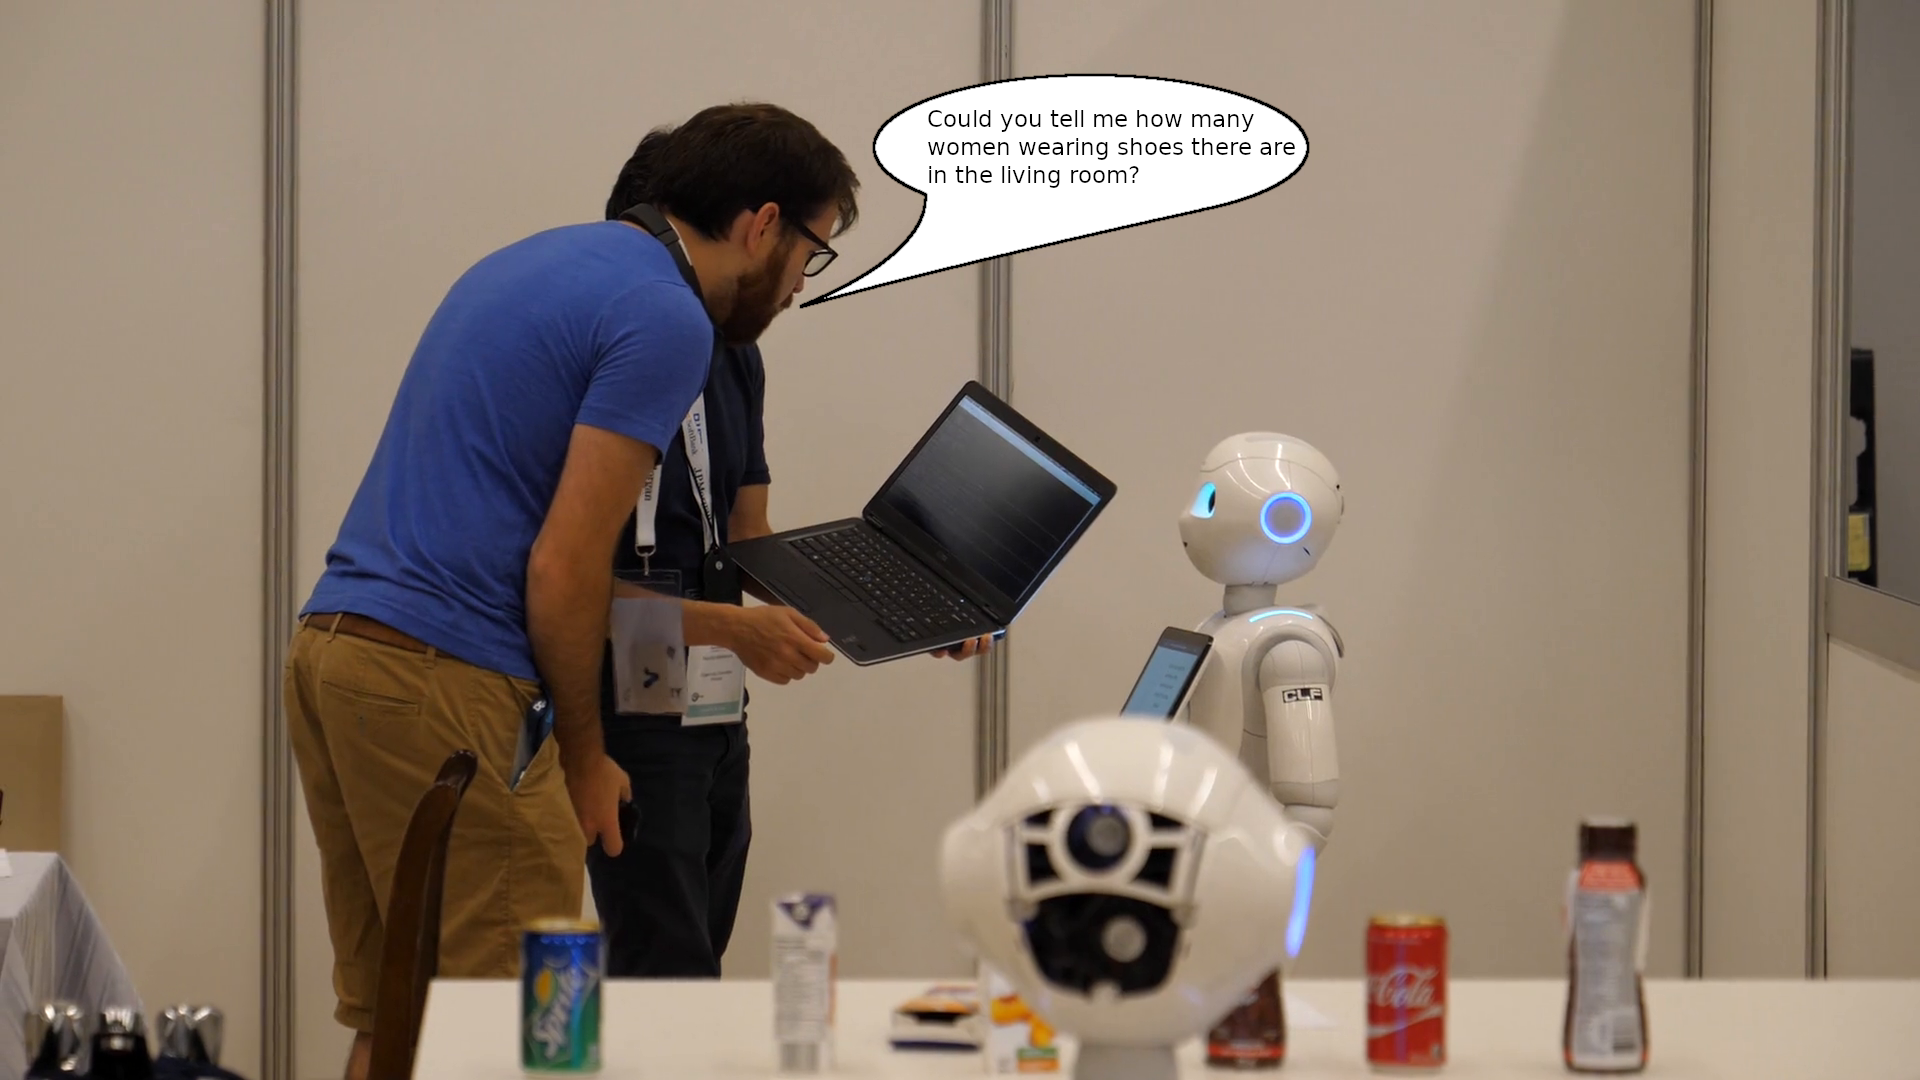
\includegraphics[width=.8\textwidth]{bilder/motivation/intro_1_edit.png}\\\vspace{3pt}
	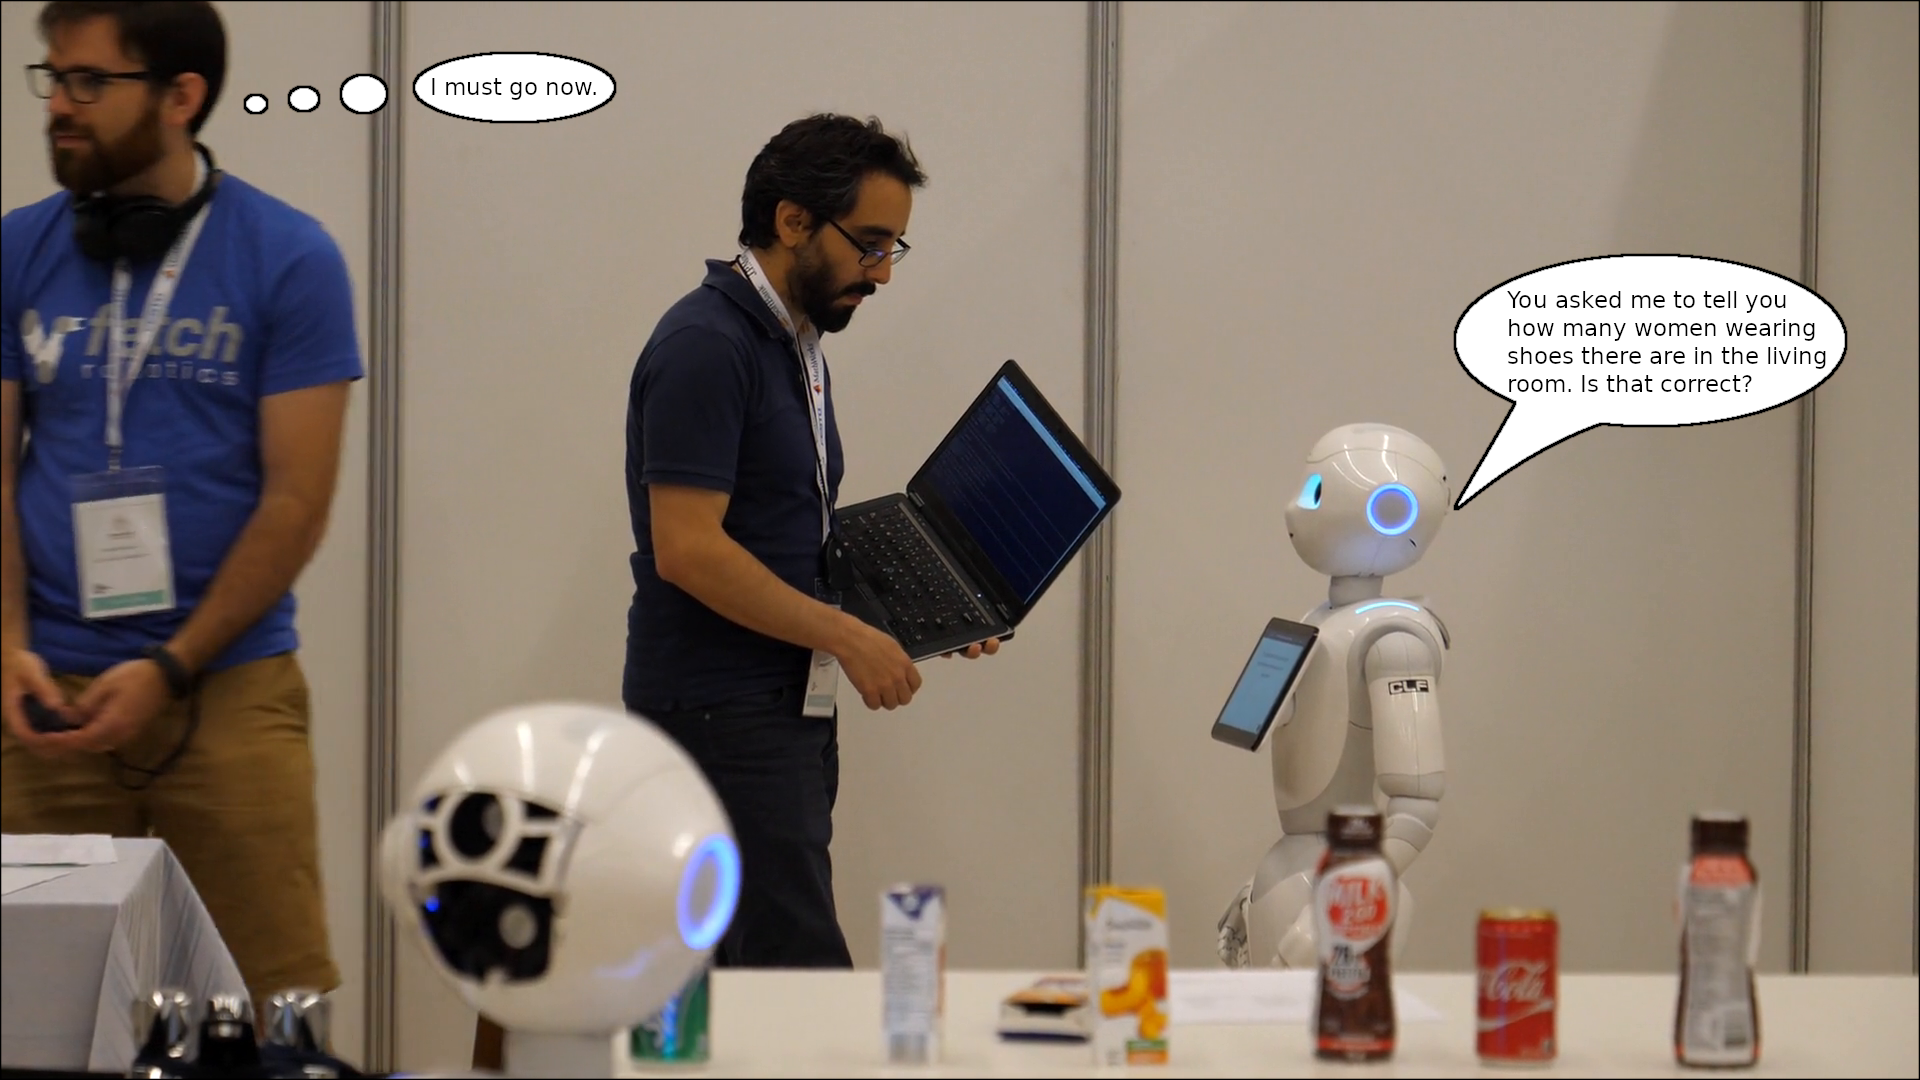
\includegraphics[width=.8\textwidth]{bilder/motivation/intro_2_edit.png}\\\vspace{3pt}
	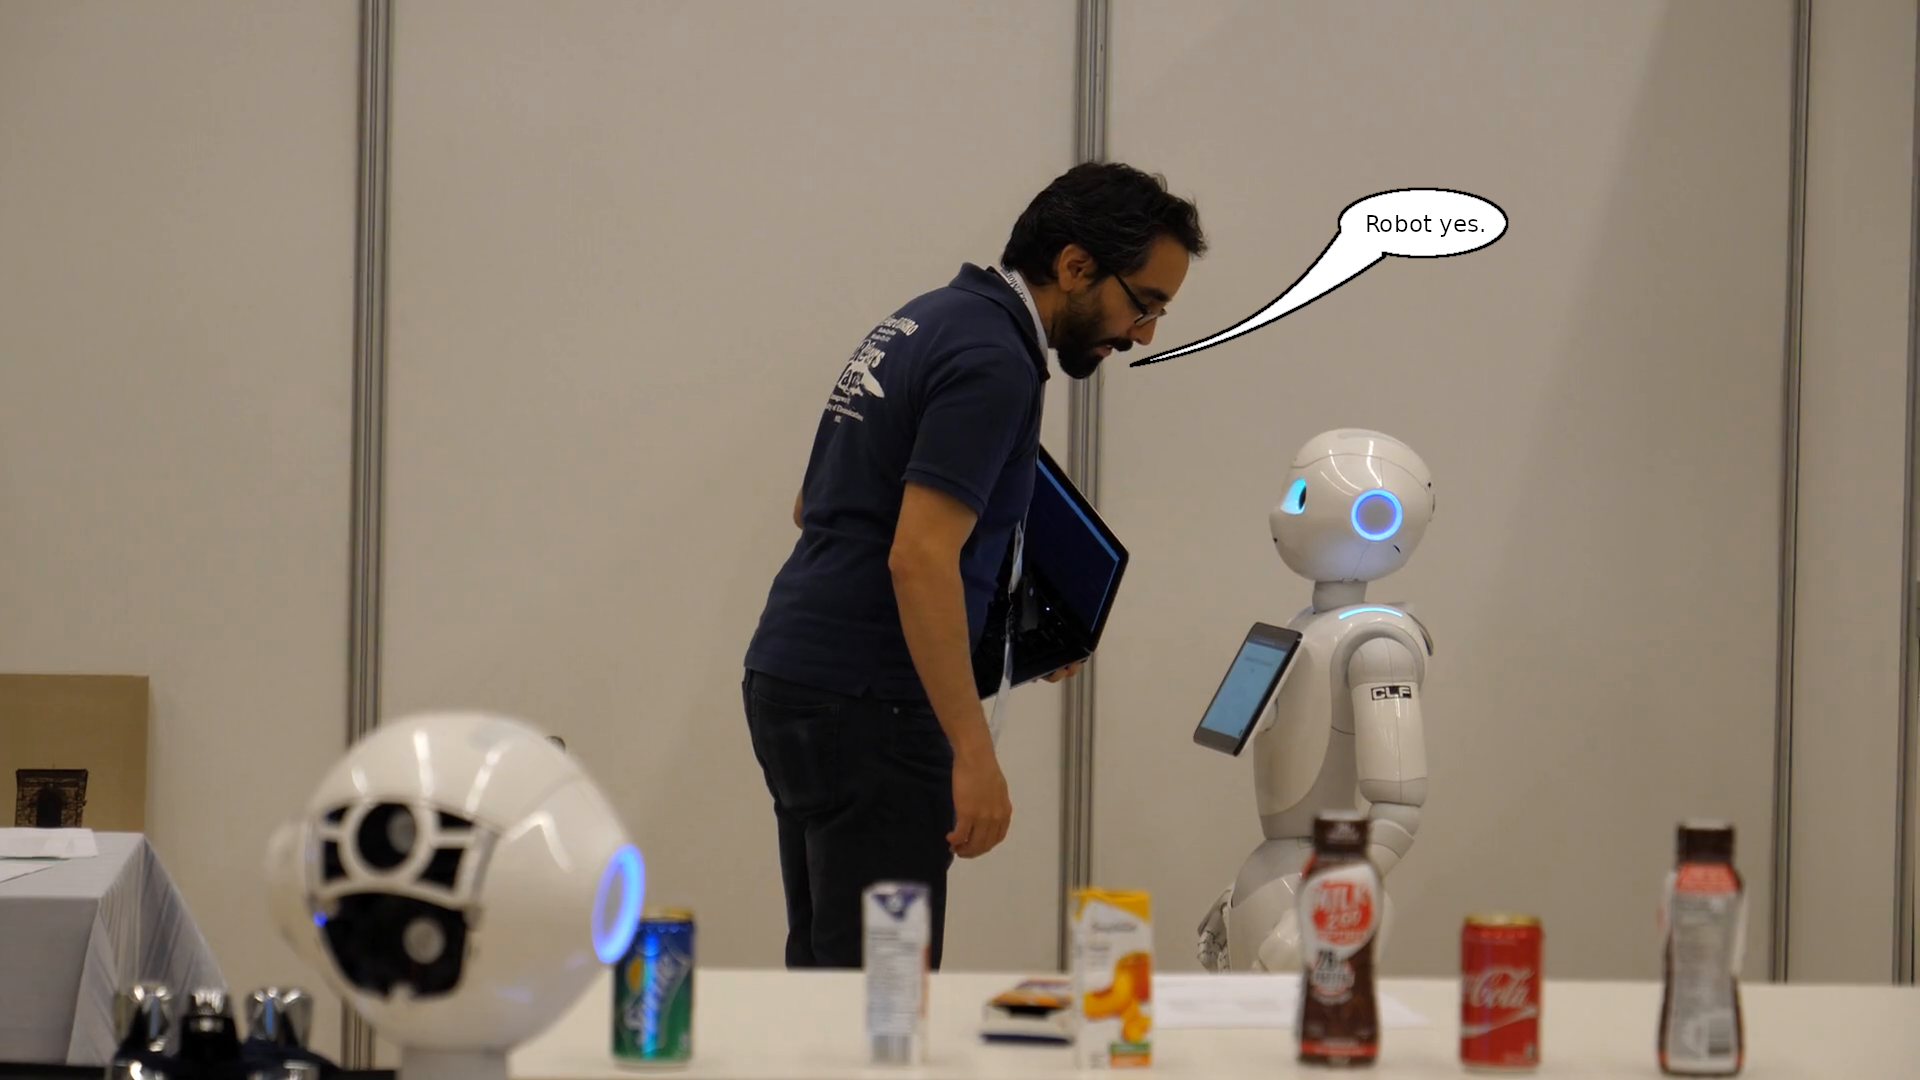
\includegraphics[width=.8\textwidth]{bilder/motivation/intro_3_edit.png}\\\vspace{3pt}
	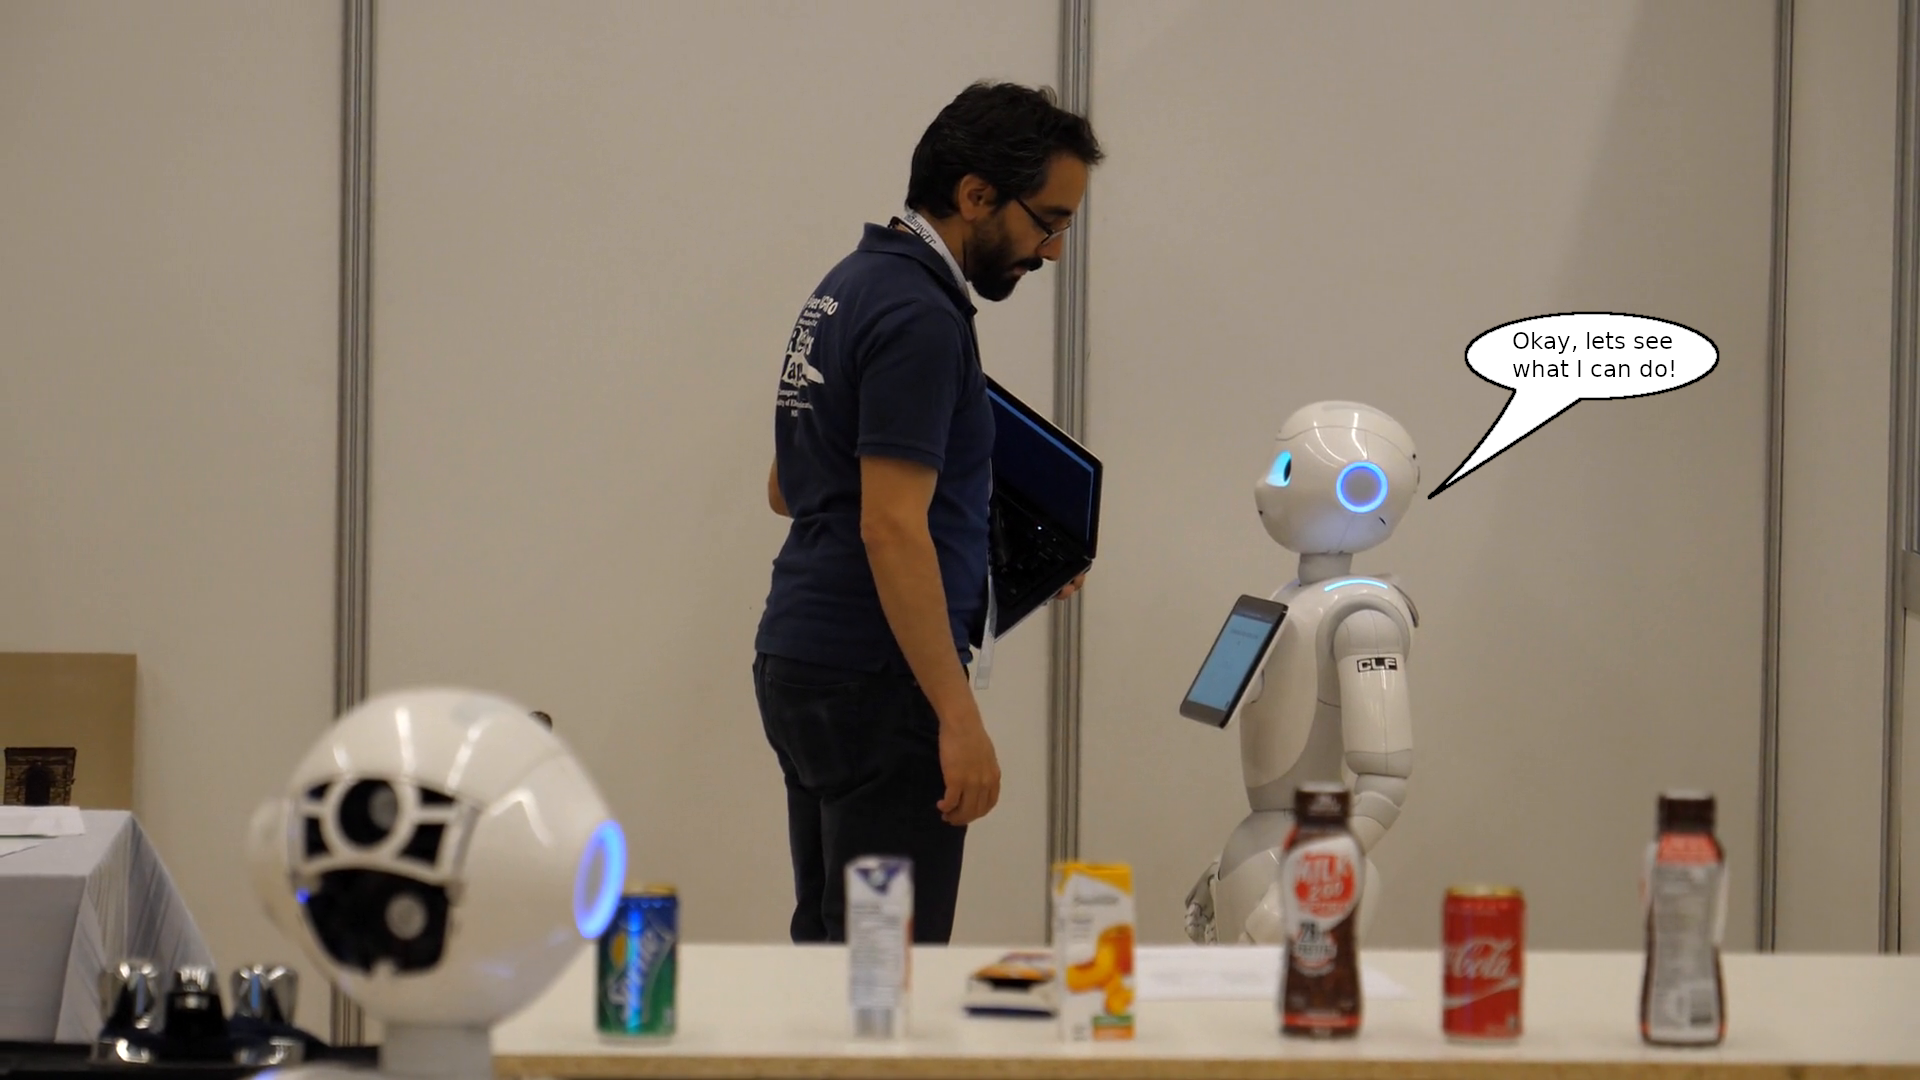
\includegraphics[width=.8\textwidth]{bilder/motivation/intro_4_edit.png}\\\vspace{3pt}
	
	\caption{Interaction between two referees and a robot in the RoboCup@home league.
		The referee in blue abandons the robot mid interaction, which does not acknowledge this at all.}
	\label{pic:moti:imustgonow}
\end{figure}

The shown interactions appear unnatural:
the robot does not seem to perceive the human, instead it is quite clear that it just listens for a particular combination of words.
A similar phenomenon could very publicly be observed in the near past, when Amazons Alexa ordered a variety of objects online, after hearing commands from a  TV commercial\footnote{\url{http://archive.is/zXuJu}}.
The solution employed by Amazon to stop this from happening with its own TV commercials seems to be a purposefully altered audio signal\footnote{\url{http://archive.is/d3uVu}} instead of a more general approach.

In the context of social robotics, this behavior is not desirable since approaches to partially solve these problems can be found in current literature \cite{opdenAkker:2009:YAR:1708376.1708379}.
Voice recognition technologies which can be used to differentiate speakers are available \cite{DBLP:journals/corr/abs-1003-4083}.
Additionally, computer vision is used to search for speakers, either standalone, looking for moving lips, or in combination with sound source localization (see \ref{basics:ssl}) \cite{1048137,lookwhostalking,840663,whosaidthat}.
We will later show (see chapter \ref{related:robocup}) these to not be used by leading robotics teams.

Suitable robot behaviors need to be created, to take all this information into account.
When creating these behaviors, one must consider how the corresponding percepts are processed.
The behavior in question must either be able to combine the information, e.g. a spoken utterance and a distinct, detected voice or receive these in a pre-combined manner.
If the behavior handles the combination, both may not be fed into the behavior at the same time, resulting in the problem to combine them.
A number of factors have to be considered when combining these information.
Information may arrive asynchronous.
For example: While just a single, long speech utterance may be received, a number of voices can be detected, or several results of the same voice.
Thus results have to be combined in a manner that takes this asynchrony into account.
Additionally, results will have different calculation times, based on what component created them and thus may be temporally unaligned.
This must be considered as well, creating the need to synchronize results based on their occurrence in time.

The problems just presented are clearly out of scope for robot behaviors an thus should be handled separately.
We thus declare the \textbf{main goal of this thesis} to create a \textbf{framework for the automatic generation of these synchronized audio analysis results}.

Furthermore, a number of \textbf{secondary goals} can be declared.
Naturally any approach to synchronize audio results shall not have a negative impact on these results.
This can be specified in two more concrete terms.
First and foremost, the \textbf{accuracy of the results shall not decrease} by being incorporated in the proposed solution.
Second, synchronizing the \textbf{results shall not take considerably longer to compute} than not synchronizing them.
To put this into context: waiting for a result more than twice as long can not be deemed acceptable.

%---------------------------------- modularity secnd goal

Robotics is a field of intensive current research, and in the last years a number of leaps have been made.
These include, but are no limited to OpenPose \cite{cao2018openpose}, YOLO \cite{yolov3} and DeepSpeech \cite{deepspeech}.
Modularity and the ability to include such advances without the need to completely overhaul an existing system greatly decreases the time needed to incorporate such new technologies.
In turn, research speed can benefit.
We can thus declare an additional \textbf{secondary goal} in the form of \textbf{modularity}, to increase the usability of the proposed framework.

%-----------------------------------

The remainder of this thesis is structured as follows:
I will first introduce concepts and frameworks in chapter \ref{basics:start}.
These start with latency, which plays a big role in the computation times and is thus of particular interest with regards to the similar secondary goal.
After this I will discuss and explain the concepts of \gls{asr}, \gls{ssl} and beamforming, as these can yield results of interest or be used to enhance audio signals, are partially incorporated in the later evaluation and will later present a number of challenges for the design of the proposed framework.
Finally I will explain \gls{ros}, a middleware used in the later proposed framework.

Thereafter I will present related work in chapter \ref{related:frameworks}, which will be divided in three parts.
First, a brief overview of a framework which focuses on \gls{ssl} and beamforming will be given.
Then I will discuss several fusion and synchronization approaches in preparation for my approach.
Lastly an overview of current and former teams of the RoboCup@Home league, a prominent will be given, with special focus on their speech understanding and data fusion approaches.

After this I will present my solution in chapter \ref{main:main}.
Based on the goals formulated above and fusion approaches discussed in chapter \ref{related:fusion}, and in consideration of the concepts of latency and beamforming discussed in chapter \ref{basics:latency}, I will then present my approach for synchronization and fusion of speech analysis data.
This solution is a framework comprised of a library and a master component, the Orchestrator.
This chapter will close with an overview of the components developed over the course of this thesis.

I will then proceed to evaluate my proposed solution in chapter \ref{eval} based on two experiments.
The first experiment is conducted with the help of a data set, and is intended to evaluate the performance of the developed framework with regards to computation time.
The second experiment is heavily inspired by the ''Speech and Person Recognition'' Task of RoboCup@Home \cite{rulebook_2018}.
It is intended to evaluate the accuracy of the proposed framework in comparison to a pre-existing solution.
Both experiments will be able to show the main goal of this thesis to be achieved.
The data set experiment in particular will show the requested modularity.

Lastly I will summarize my findings and point out possible future work in chapter \ref{conclusion}.
The central point of this chapter is that due to the findings of chapter \ref{eval}, more and better components can be developed and the next step can be taken, i.e. behaviors equipped to handle situations such as those seen in figure \ref{pic:moti:imustgonow} by utilizing synchronized data can be created.

%In the appendix, I will detail the source code repositories as well as build and start instructions for the acrewed components.